
% ========================================================
% INTRO
% ========================================================
Being a tiny part of the \ac{CMS} collaboration I would like to start by clarifying how my experiment is integrated into the amazing project called the \ac{LHC}.
% ========================================================
% LHC
% ========================================================
\section{\ac{LHC}}
The LHC is the most powerful high energy particle accelerator that has ever been built on earth. The collider is located in a circular tunnel of $26659\,$m in circumference, which covers an area of an area of $56.6\,$km$^{2}$ and is underneath the territory of \ac{CERN}. It crosses the border between Switzerland and France and is close to the Swiss city Geneva. The accelerated particles are exclusively protons that are colliding with a \ac{COM} energy of $14\,$TeV \cite{lhc}.
% ========================================================
\subsection*{Accelerator Complex}
In order to increase the energy of the protons from a few keV (kinetic energy) at room temperature up to $7\,$TeV a succession of machines is required of which each increases the energy more and injects into another until it finally reaches the last iteration, the \ac{LHC}. A schematic of the whole procession can be found in \ar{p18}.\\
The protons are coming from an ordinary bottle of compressed hydrogen, whose molecules are stripped of their electrons in the source chamber of the linear accelerator LINAC2 where they are accelerated to $50\,$MeV using radiofrequency cavities. Leaving LINAC2 the particles are injected into the first circular accelerator, the \ac{PSB} and are accelerated up to $1.4\,$GeV, which is already equivalent to $91.6\%$ of the speed of light. After that \ac{PS} and \ac{SPS} increase their energy further to $25$ respectively $450\,$GeV. Once the protons leave \ac{SPS} they are injected both clockwise and anti clockwise into the ring of \ac{LHC} where they reach their final energy of $7\,$TeV within approximately $20$ minutes. They are now over $7000$ times heavier than at rest at $99.9999991\%$ of the speed of light.\\
At \ac{LHC} there are six experiments installed: \ac{CMS}, \ac{ATLAS}, \ac{LHCb}, \ac{ALICE}, \ac{LHCf} and a \ac{TOTEM} of which the first four are in underground caverns around the interaction points. \ac{TOTEM} is close to the interaction point of \ac{CMS} and \ac{LHCf} is near \ac{ATLAS}.
\begin{figure}[ht]
	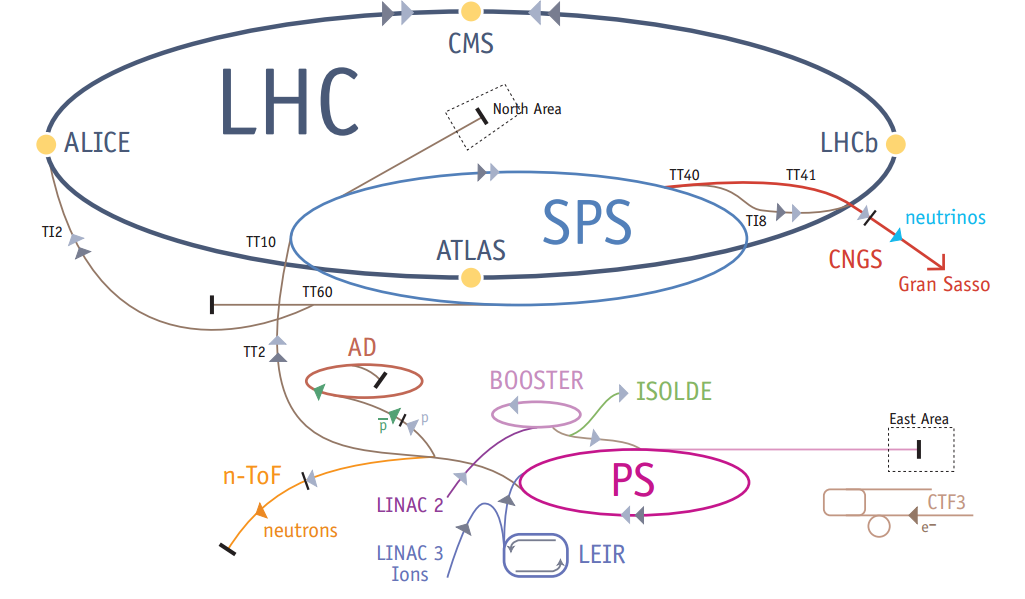
\includegraphics[width=0.95\textwidth]{lhc}
	\caption{Schematic of the \ac{LHC} accelerator complex \cite{lhc}.}
	\label{p18}
\end{figure}
% ========================================================
% CMS
% ========================================================
\section{\ac{CMS}}
\ac{CMS} belongs together with \ac{ATLAS} to the two general experiments at \ac{LHC} and is located beneath the French town Cessy. Its main goals are the study of the properties of the recently found boson (assumed to be Higgs) and the search for evidence of physics beyond the standard model, in particular \ac{SUSY} and extra dimensions. The name \ac{CMS} derives from its design, which is rather small compared to other detectors of its capability, has an excellent ability to measure myon tracks and it has a unique, very strong solenoid magnet.\\
A sectional view of the detector is shown in \ar{p19}.
\begin{figure}[ht]
	\centering
	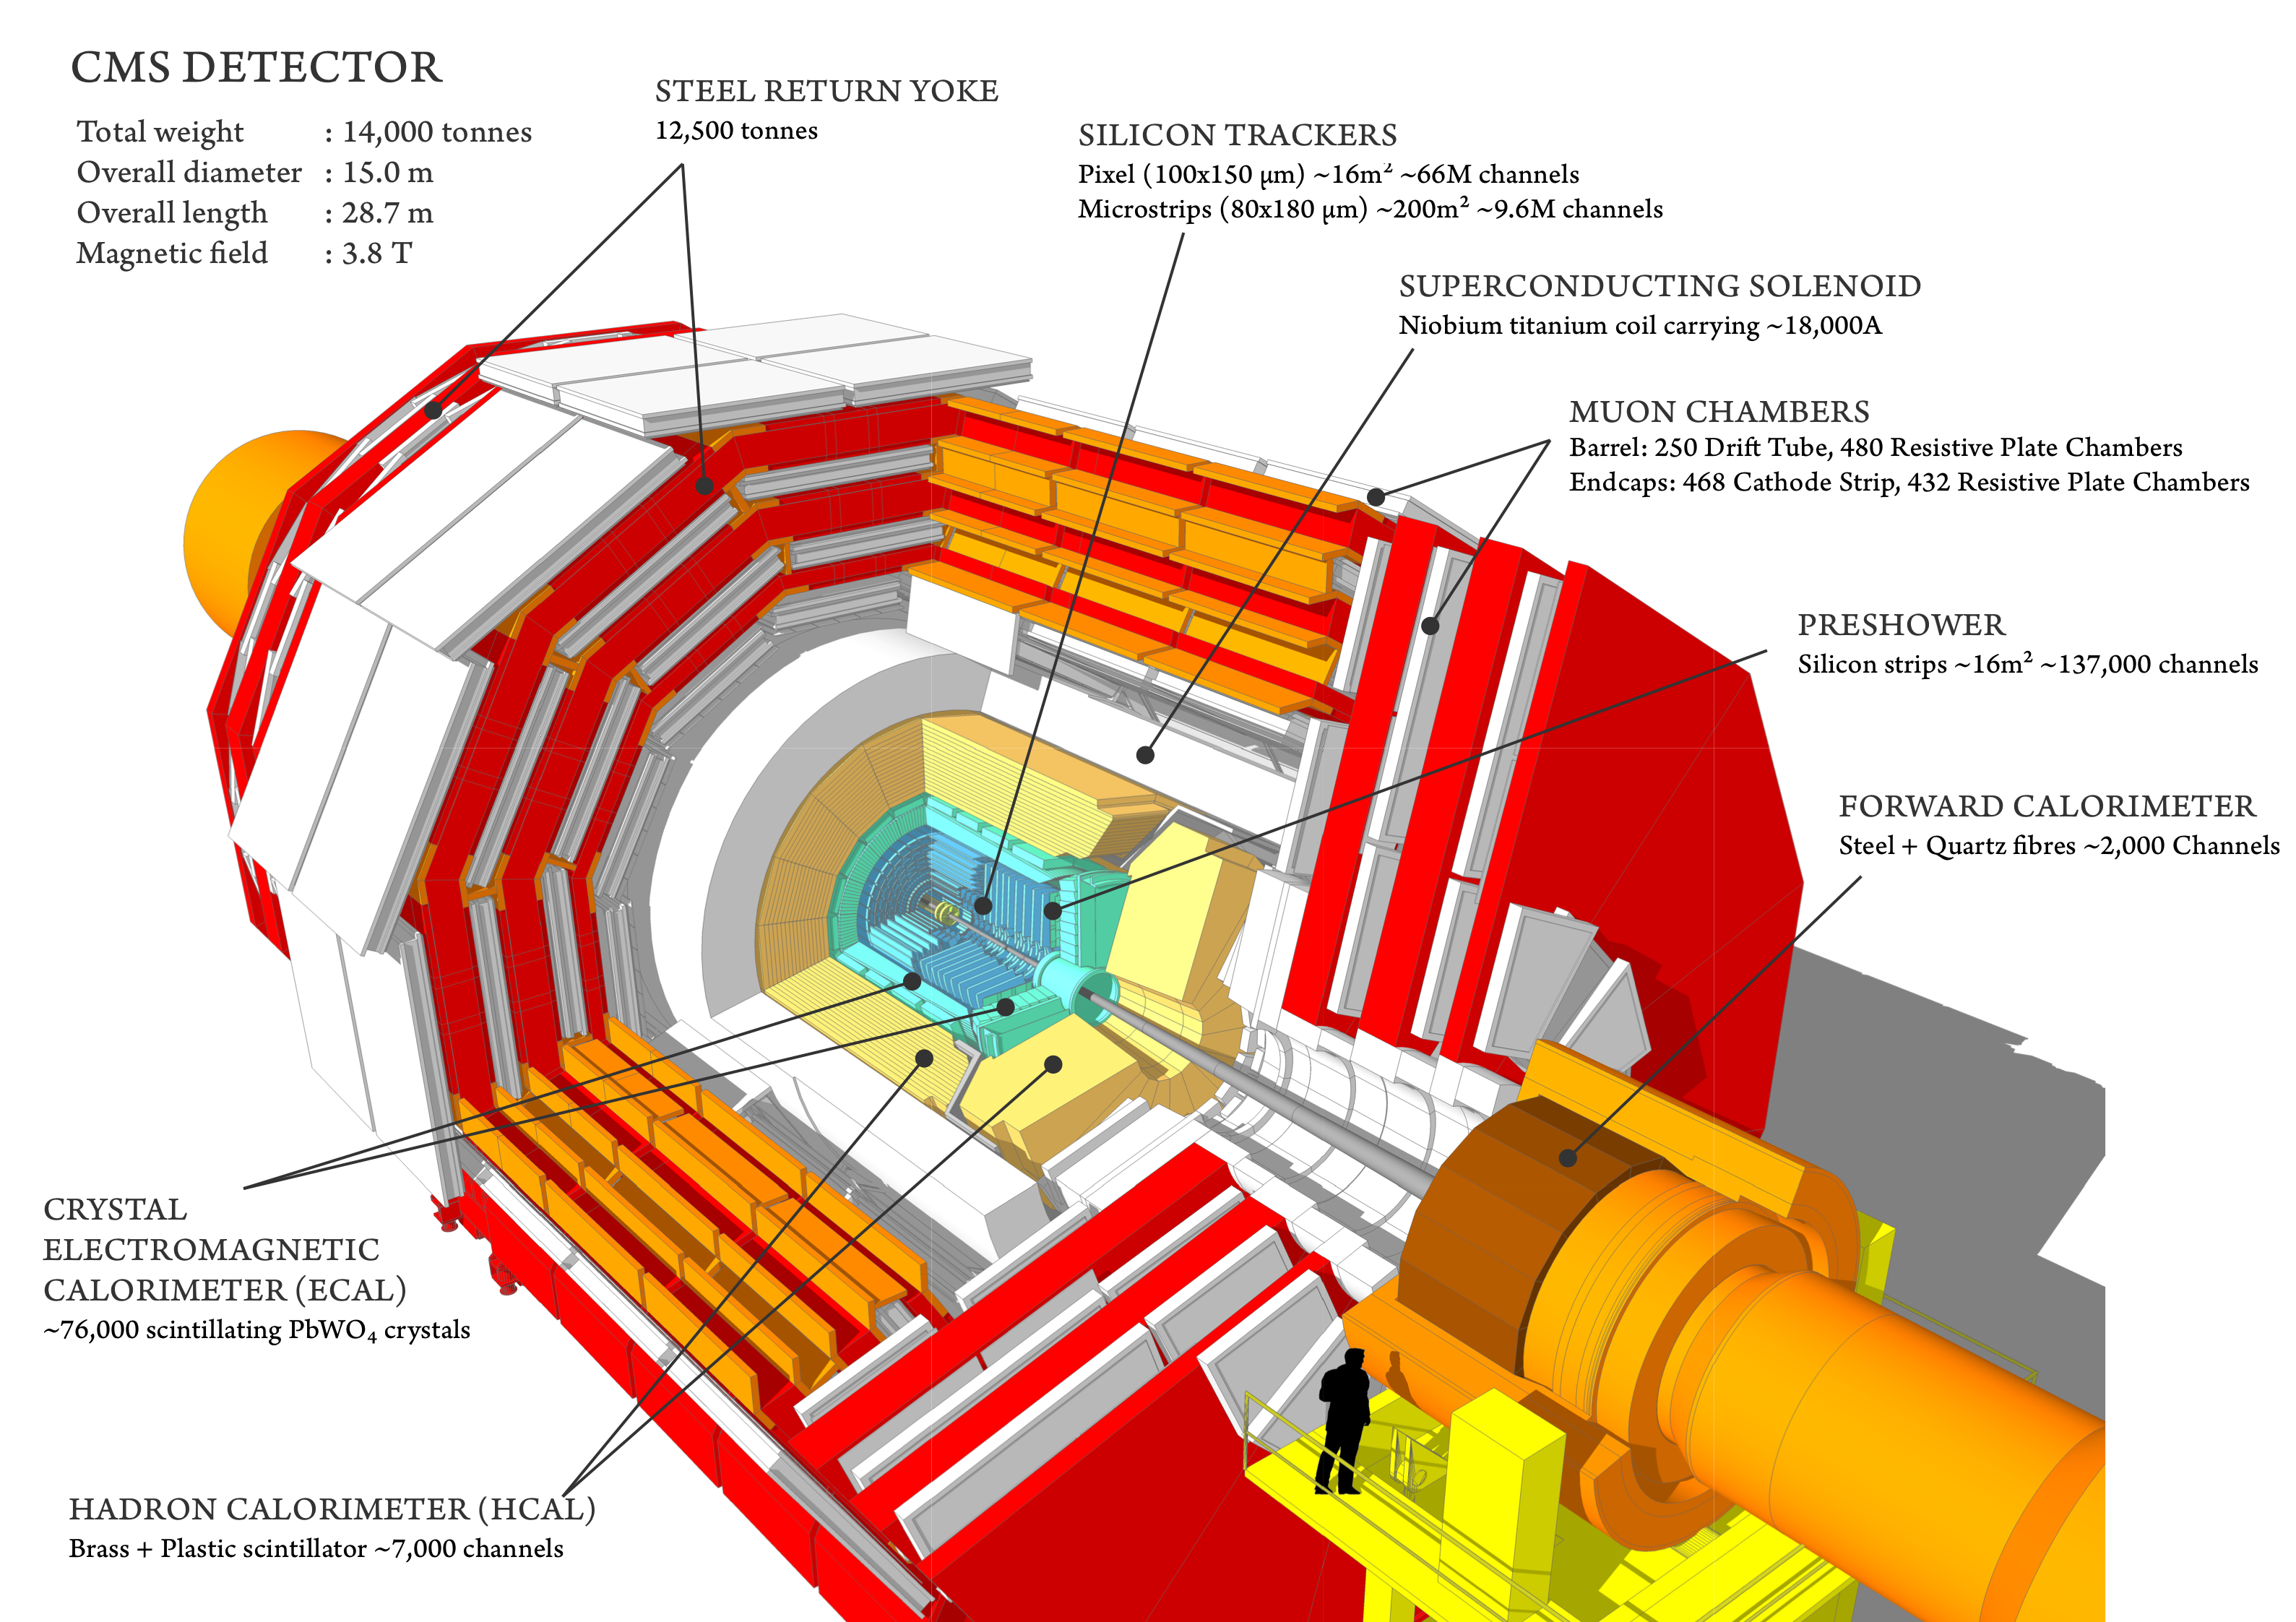
\includegraphics[width=0.95\textwidth]{cms_cut}
	\caption{Sectional view of the CMS detector.}
	\label{p19}
\end{figure}
% ========================================================
\subsection{Solenoid}
The shape of the solenoid strongly determined the whole design of the detector. A solenoid is magnet of coils that are tightly wound into helices and that have uniform magnetic field inside of the helix, once constant electric current flows threw the wires. Its purpose is to bend the paths of the particles that are created at the interaction point. It was aimed to be the strongest possible magnet because the stronger the magnetic field, the smaller the bending ratio of the particle gets, which in the end increases the momentum resolution of the tracker. To reach a final magnetic field strength of $4\,$Tesla the whole magnet is brought down to a temperature of $-268.5\,^{\circ}$C to guarantee superconductivity. Interestingly, particles with an energy of less than $1.6\,$GeV will circle inside the detector and will traverse to the end caps on a helical trajectory without ever reaching the calorimeter. 
% ========================================================
\subsection{Tracker Detector}
The main goal of the Tracker Detector is to measure the momentum of passing particles to be able to get an idea of the incidents during the collision. The momentum is calculated the track through the magnetic field the solenoid provides. The \ac{CMS} tracker then records the path of the charged particle by finding its position at a number of key points. That way it is possible to precisely reconstruct paths of long living particles such as muon, electron or hadrons, but also see the tracks of short living particles like the beauty quark.\\
For the whole experiment is very important to measure precise tracks on the one hand as well as to have as less disturbing of the particles as possible. That is one reason why only a certain number of points are measured for the tracking, which was accomplished building several layers around the beam line.\\
The innermost layer of the detector is located but $4\,$cm away from the interaction point where a detectors are exposed to an approximate particle flux of $100\,$Mhz\,cm$^{-2}$. That is why one of the most important properties of the detector has to be radiation hardness. As the current detector was built, it was decided to build it completely out of silicon. To be able to deal with the high number of particles the inner layers are made of pixel detectors whereas the outer ones more than $20\,$cm away from the interaction are made out of strip detectors.
% ==========================
\subsubsection{Pixel Detector}
Though only roughly the size of a shoe box, the Pixel Detector at \ac{CMS} contains $65$ million single pixels. They are arranged in three layers of barrel modules $4\,$cm, $7\,$cm and $11\,$cm away from the beam and two disks at either end (q.v. \ar{p22}). This system is able to reconstruct the tracks of ten million track per second and was build to withstand the duration for an operation time of ten years up to the Phase 1 Upgrade. Due to the huge amount of pixels it import keep the power consumption of the pixels at a minimum. Although they only need $50\,\upmu$W per pixel they are still mounted on cooling tubes so that the detector will not overheat.\\
The \ac{CMS} Pixel Detector is also the most important part concerning my thesis and is explained in further detail in \ar{s130}.
\begin{figure}[ht]
	\centering
	\begin{subfigure}[b]{0.47\textwidth}
        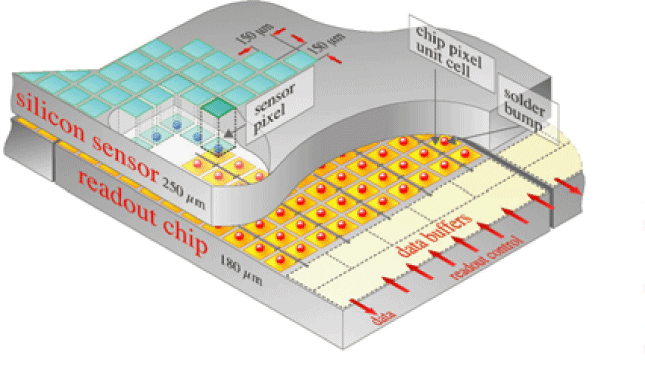
\includegraphics[width=\textwidth]{pixelement}
		\caption{\ac{CMS} silicon pixel detector}
		\label{p21}
	\end{subfigure}
	\hfill
	\begin{subfigure}[b]{0.47\textwidth}
		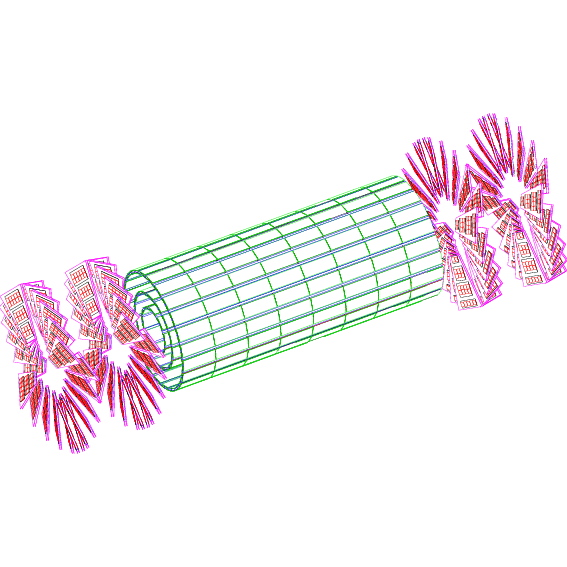
\includegraphics[width=\textwidth]{barrel}
		\caption{Pixel layers around the beam line.}
		\label{p22}
	\end{subfigure}
	\caption{Schematics of the pixel detector.}
	\label{ppixdet}
\end{figure}
% ==========================
\subsubsection{Strip Detector}
Right after the three pixel layer follow ten layers of strip detectors up to a radius of $130\,$cm. A schematic of the way they are placed is shown in \ar{p23}. First come four inner barrel layers with two inner endcaps. After that follow the outer layers: two double sided and four one sided barrel layers. Altogether the tracker detector consist of $10$ million silicon strips, which have the same working principle as the pixel detectors even though different chips are used for the readout. To keep radiation damage at a minimum the whole system is cooled down to a temperature of $-20\,^{\circ}$C.
\begin{figure}[ht]
	\centering
	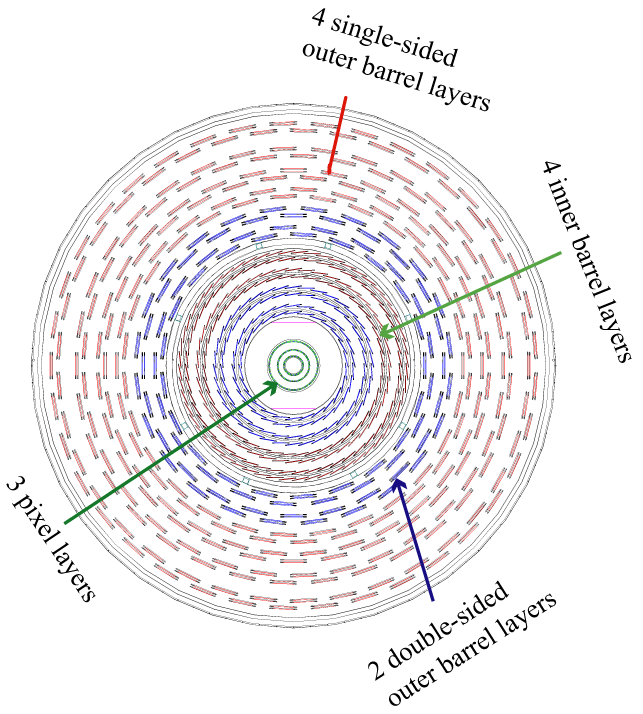
\includegraphics[width=0.4\textwidth]{strip}
	\caption{Tracker layers perpendicular to the beam.}
	\label{p23}
\end{figure}
% ========================================================
\subsection{Calorimeter}
In particle physics a calorimeter is a device to measure the full energy of particles. When a particle enters the detector material a chain reaction called particle shower is started until the incident particle has deposited all its energy in the calorimeter. In many cases the detectors have transverse segmentation to provide information about the direction of the particle and longitudinal segmentation to get information about the identity of a particle by the shape of the shower. Since electrons and photons interact very differently with matter at the same energy as hadrons two different types of calorimeters are required: the \ac{ECAL} and the \ac{HCAL}.
% ==========================
\subsubsection{\ac{ECAL}}
The \ac{ECAL} consists of $75848$ lead tungstate crystals (PbWO$_{4}$), which is a scintillating material and has with its short radiation length, narrow showers and its good radiation hardness excellent properties to function in such an environment. Glued on top of the crystals are photodetectors that collect the light, amplify it and transform it into into a electric signal that is then sent to analysis.
% ==========================
\subsubsection{\ac{HCAL}}
The \ac{HCAL} is built to measure hadrons which consist out of quarks and gluons. It was designed to be as hermetic as possible, i.e. to stop every particle from the collision in order to be able to draw conclusions about missing transverse energy. It is a so called sampling calorimeter which means that it finds the position, energy and arrival of a particle by using repeating layers of a dense brass absorber and plastic scintillators. The \ac{HCAL} is the last part of the detector that is placed inside the solenoid.
% ========================================================
\subsection{Muon Chambers}
Outside of the solenoid are the muon chambers, since muons can penetrate very dense material for several meters without interacting at all. They are produced as decay products of many particles including potential new ones and thus play an import role as signals that can be triggered on. The whole muon detector consists of $1400$ muon chambers that split up into $250$ drift tubes and $540$ cathode strip chambers that track the particles and provide a trigger and $610$ resistive plate chambers that form a redundant trigger system, which decides weather to keep the data or not.\as 
A diagram of all parts and the positioning within the \ac{CMS} detector is shown in \ar{p20}. It also demonstrates how typical particles will behave passing through the various steps.
\begin{figure}[ht]
	\centering
	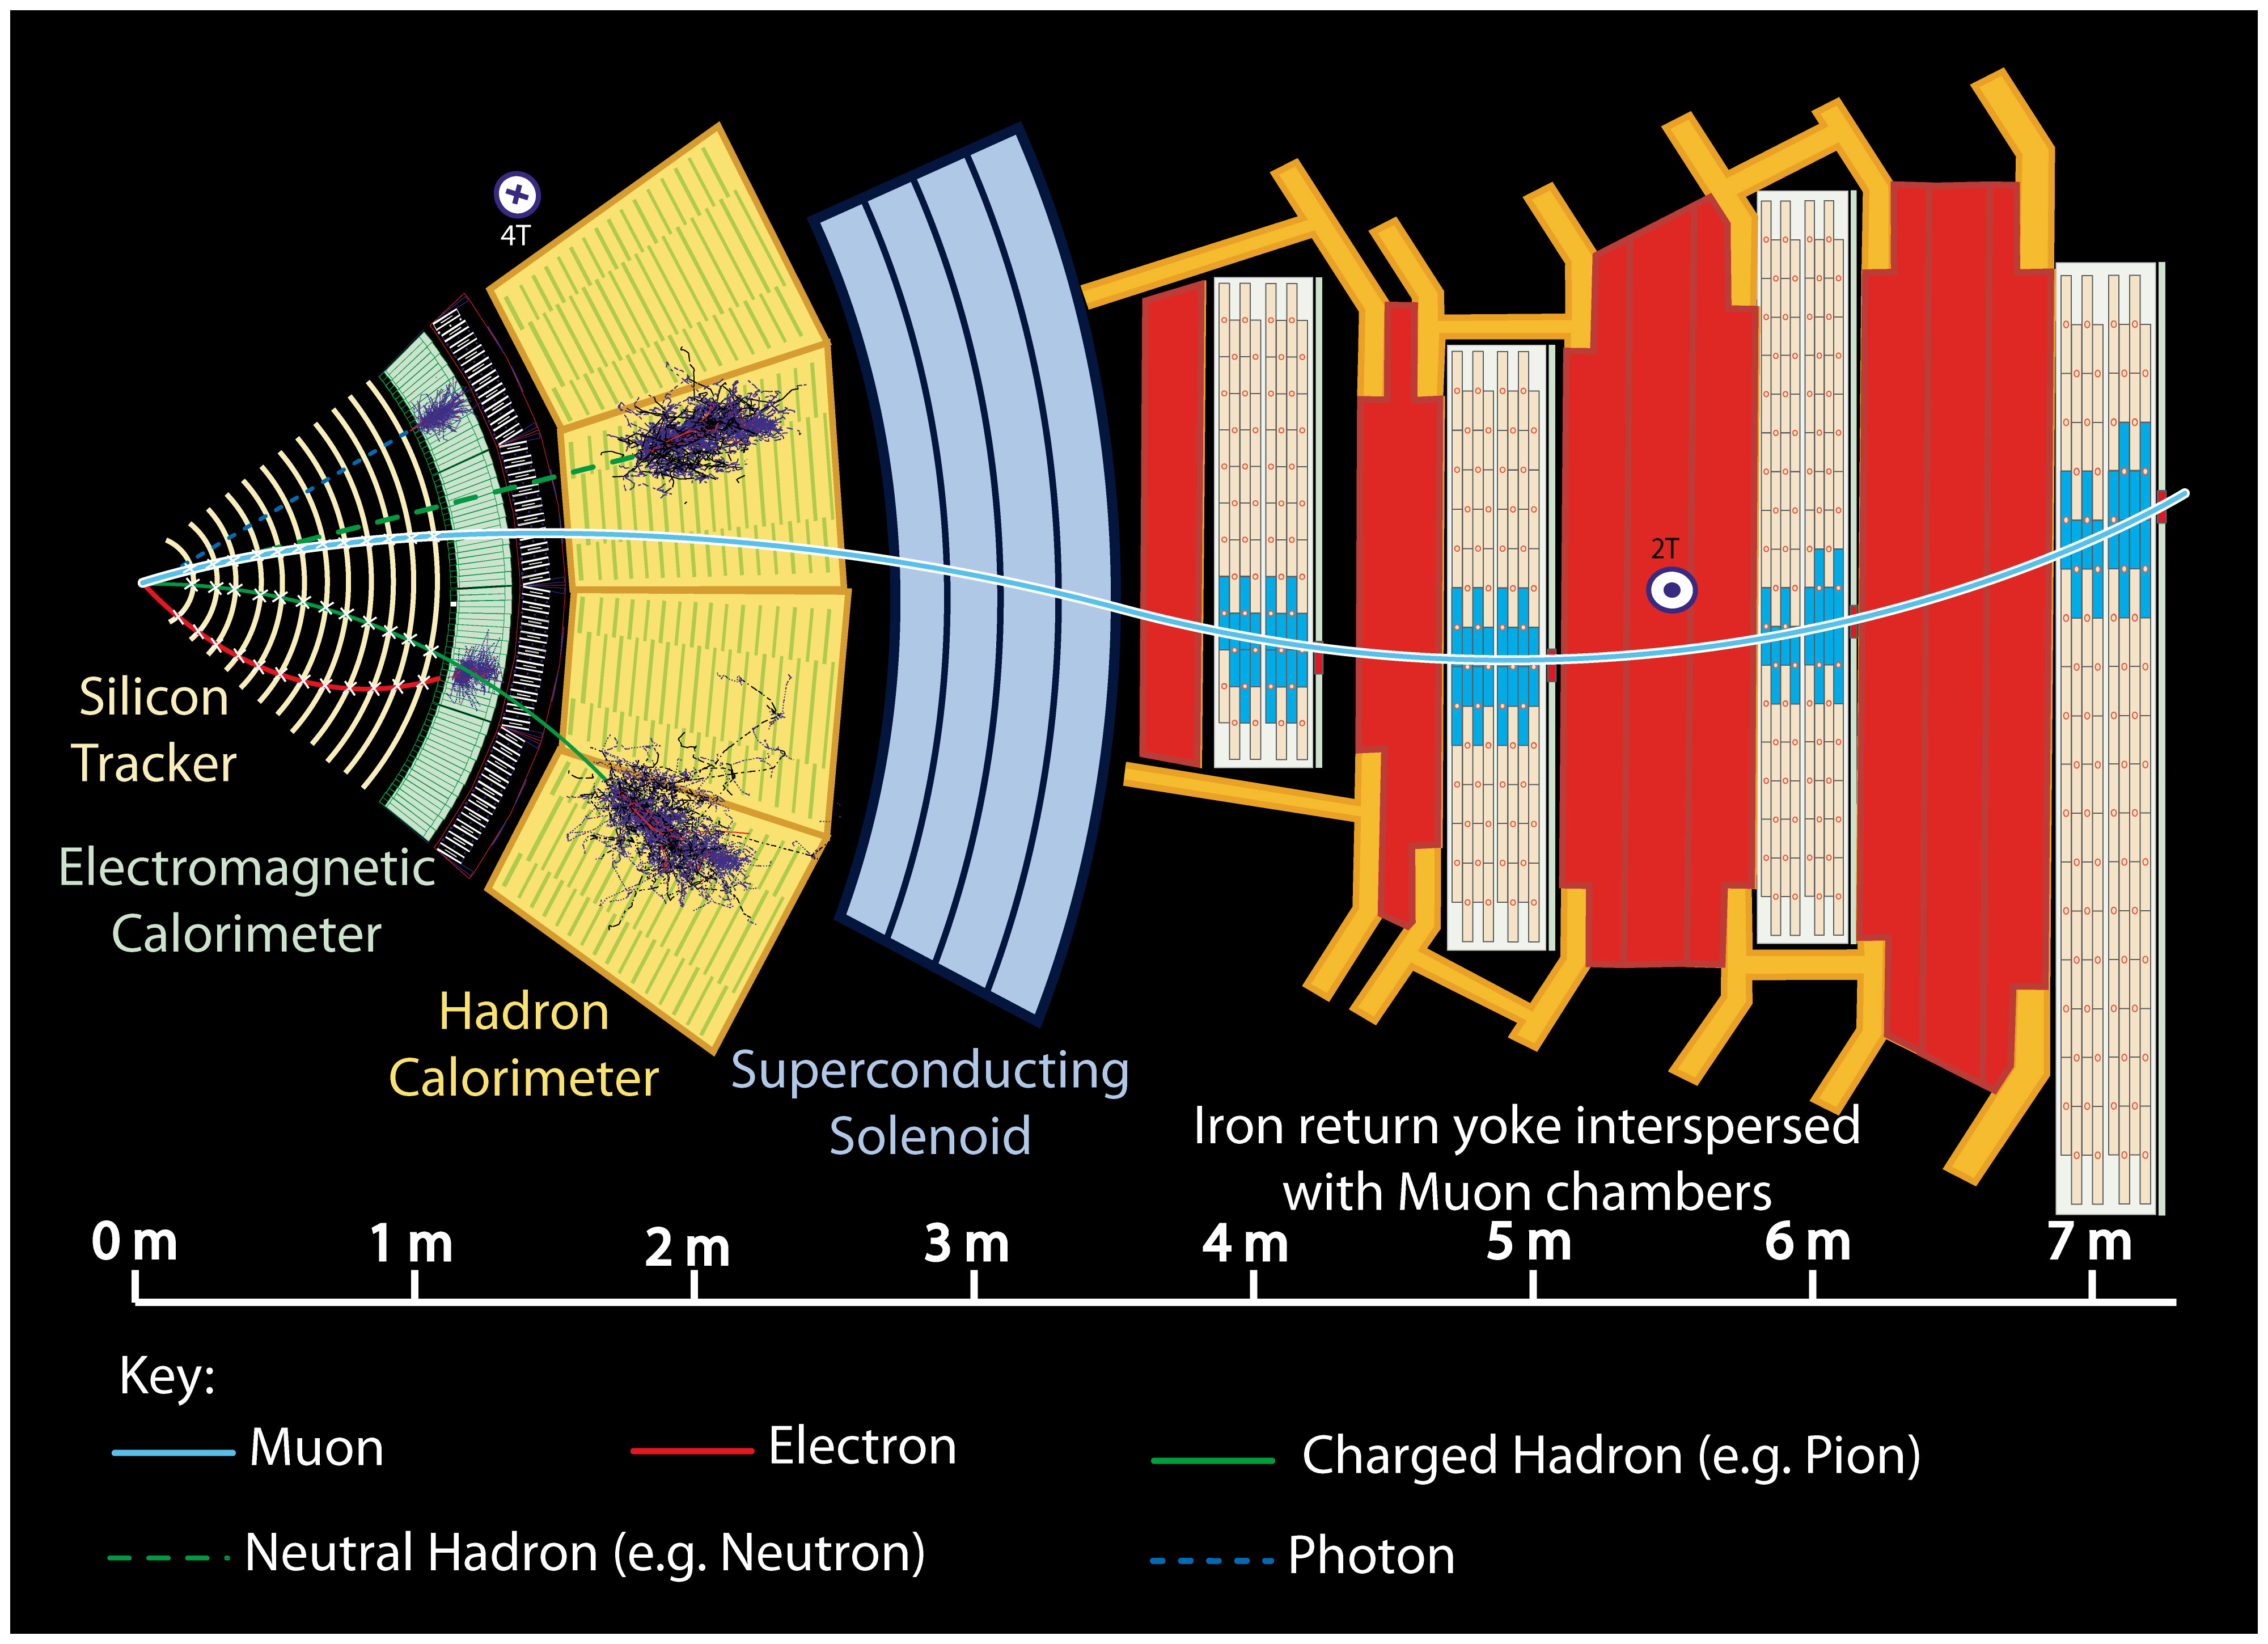
\includegraphics[width=0.95\textwidth]{cms_slice}
	\caption{Sliced view of the CMS detector with tracks of various particles.}
	\label{p20}
\end{figure}
% ========================================================
\subsection{Trigger System}
With almost a billion interactions per second it is almost impossible to save or even analyse every single event. That is why a trigger is required to save only the interesting events. Since there are collisions every $25\,$ns the data is stored in pipelines with precise timing information for a short time. In order not to information from different events it all the streams of one event have to be synchronised. \\
The first step to reduce the huge amount of information is called the level 1 trigger, which is a full hardware trigger, that decides within $3.2\,\upmu$s if the event could contain interesting physics based on information of the calorimeter and the muon chambers. These are events with large amount of energy or unusual combination of particles for example. This trigger already reduces the number of events per second to $100000$. In the next step, the high level trigger, the whole event is recreated and the information sent to computers to pre-analyse it, which makes it a full software trigger. In the end only $100$ events per second are considered interesting and will be saved.\\ 
The level 1 trigger of \ac{CMS} is interesting because it has direct connection to the trigger system I was using. 
% ========================================================
% CMS Pixel Chip
% ========================================================
\section{CMS Pixel Chip}\label{s13}
All pixel chips that are currently in use at \ac{CMS} are analogue silicon chips, which means that their output data format is an analogue signal. During the Phase 1 Upgrade it is planned to exchange all of them with a more efficient silicon digital chip. Due to the increase of the luminosity and \ac{COM} energy there has even been the notion to add fourth layer of pixel chips and use diamond pixel chips for the innermost layer. Among other advantageous properties diamond is much more radiation resistant than silicon. Though, if diamonds are suited for that purpose is still under test.\\
For my thesis I was using both analogue and digital silicon chips, I was even given the chance to participate in the testing of digital diamond pixel chips. The purpose for my thesis is in parts the exact same as for \ac{CMS}: use several of them as tracking device. Additional applications will be described in the following.
% ========================================================
\subsection{Analogue Pixel Detector}\label{s130}
The analogue pixel detector was designed i.a.to precisely reconstruct hits, withstand radiation damage for several years of operation, keep multiple scattering at a minimum and avoid fake hits due noise in electronics. Each single detector consists out of $4160$ pixels in $26$ double columns and $80$ rows. The single pixels have a size of $150\,\upmu$m $\times$ $100\,\upmu$m, which adds up to a size of $7.8\,$mm $\times\ 8.0\,$mm (q.v. \ar{p24} and \ar{p21}) and corresponds to an area of a little more than half a square centimetre. The detector itself consists of two parts: a pixelated silicon sensor and a \ac{ROC}, which have both the same arrangement of pixels. They are attached to one another and electrically connected via indium bump bonds of roughly $20\,\upmu$m \cite{kaestli}. The connection from the \ac{ROC} to the readout as well as the connection to the bias voltage is made via delicate wire-bonds.
\begin{figure}[ht]
	\centering
	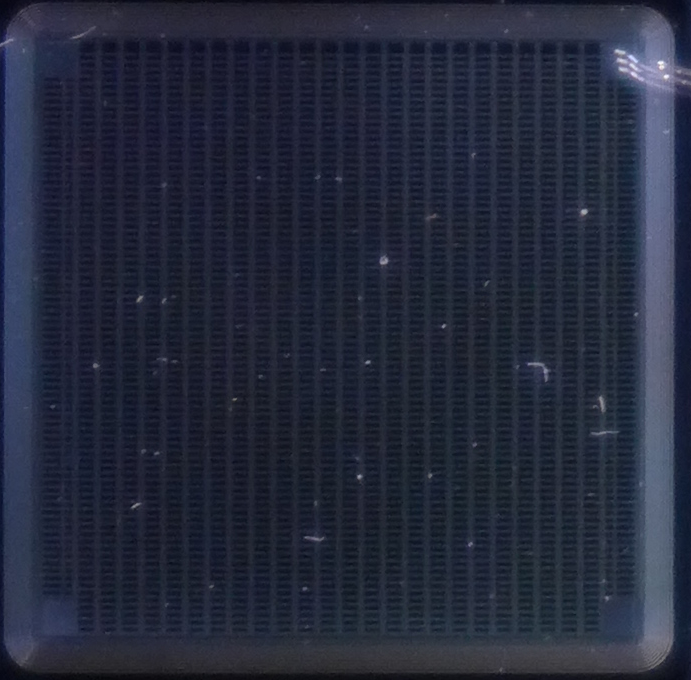
\includegraphics[width=6cm]{ROC0}
	\caption{Photograph of an analogue pixel detector}
	\label{p24}
\end{figure}
% =======================
\subsubsection{Sensor}\label{s220}
For the current detector silicon was chosen as sensor material. The average energy to create an electron-hole pair in silicon is $3.6\,$eV. By applying a bias voltage to the sensor the charge carriers are moved to the collecting electrode and a signal can be measured. The silicon sensor itself consists of high-dose n-implanted pixels introduced into a high resistive n-substrate. The backside of the sensor is p-doped and thus creates a pn-junction \cite{allkofer}. The small pixel size was chosen to get a good spatial resolution. The thickness of the sensor is about $285\,\upmu$m which means that minimum ionising particles will most probably create approximately $22000$ electron-hole pairs\footnote{The energy is loss is Landau distributed. This value is equivalent to the peak value of this distribution (q.v. \ar{makeref})} in the sensor. In order to deplete an unirradiated sensor of that thickness completely one has to apply a bias voltage of roughly $100\,$V \cite{pixadd}. For irradiated detectors that value may be up to four times higher.
% =======================
\subsubsection{\ac{ROC}}\label{sroc}
The \ac{ROC} has of two parts: An active part consisting out of $26$ double columns of $2\times80$ \ac{PUC}s matching the pixels of the sensor and a periphery consisting of a control interface and a data buffer, this is depicted in \ar{p8}. In order for the \ac{ROC} to record data, handle triggers and be read out the buffer splits up into four different counters:
\begin{enumerate}
	\item $8\,$bit bunch crossing counter - time stamp in the timestamp buffer
	\item $8\,$bit bunch crossing counter with trigger delay - runs a number of counts behind the bunch crossing counter (adjustable by \ac{DAC} wbc)
	\item $4\,$bit trigger counter
	\item $4\,$bit token counter
\end{enumerate}\par
The periphery is the reason is why the \ac{ROC} is with $7.9\,$mm$\times\ 9.8\,$mm 
\begin{wrapfigure}{l}{8cm}
	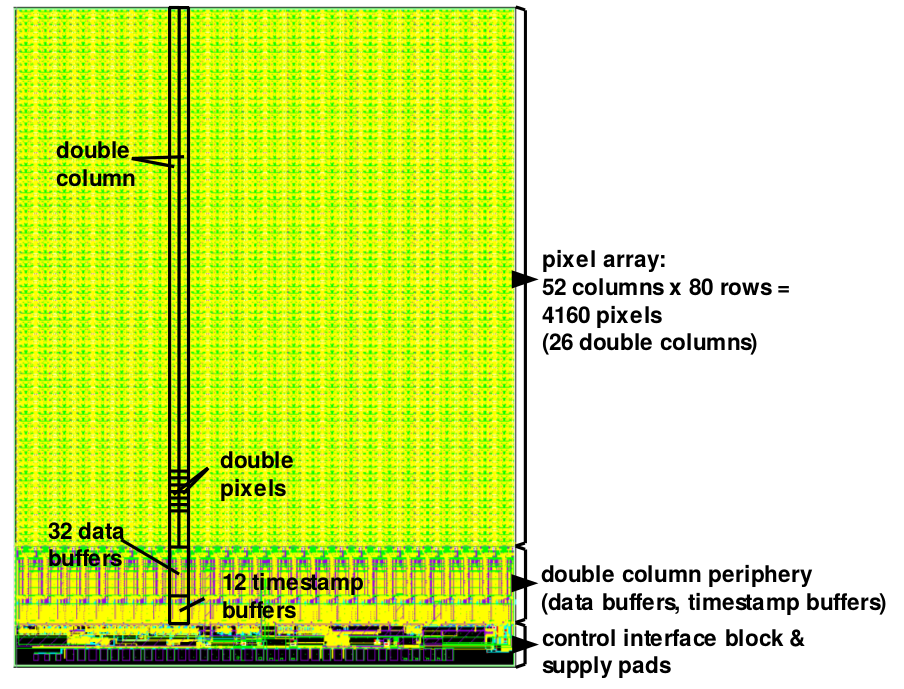
\includegraphics[width=7.9cm]{ROC_scheme}
	\caption{schematics of a \ac{ROC} \cite{psi46chip}}
	\label{p8}
\end{wrapfigure}  
a few millimetres longer than the sensor. The \ac{ROC} is programmable with a set of  $26$ \ac{DAC} values (q.v. \ar{t0}) that are required to control its behaviour, since every \ac{ROC} differs from another and they have to be comparable. More details about the \ac{DAC}s can be found in \ar{sdacs}. In order to maintain the \ac{ROC} at constant temperatures it also equipped with a temperature sensor.\\
If a particle hit creates electron-hole pairs in the sensor a voltage signal is induced in the corresponding \ac{PUC}. A schematic of a \ac{PUC} is shown in \ar{p9}. Once a signal enters the \ac{PUC} it gets amplified and shaped. If it exceeds a certain threshold, which is tunable with one the \ac{DAC}s, it will be send to the periphery. The pixel information and the bunch crossing are then stored in the buffer for each double column. The option to sent calibration signals directly to the front end of the \ac{PUC} makes it very easy to test the basic functionality of the \ac{ROC} without having any particles inducing signals. There is a switch to enable and disable sending these calibrates for every pixel.\\
Furthermore, an important feature of the analogue \ac{ROC} is the so called fast-OR. Every time the threshold of a single pixel is exceeded the \ac{ROC} sends out this signal. It is an logical OR of all pixels of the \ac{ROC} and its shape gives conclusions distribution of hit pixels (q.v. \ar{makesection}). It is very useful as trigger signal for other devices or as self trigger.
\begin{figure}[ht]
	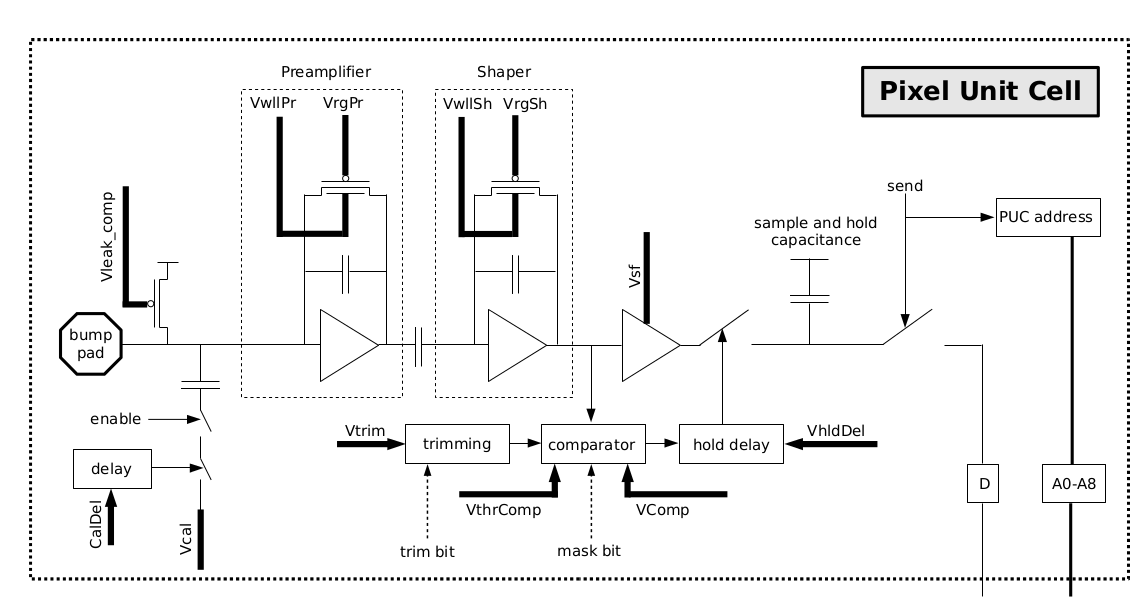
\includegraphics[width=0.95\textwidth]{PUC}
	\caption{schematic view of a \ac{PUC} \cite{dambach}}
	\label{p9}
\end{figure}
% =======================
\subsubsection{\ac{DAC}s}\label{sdacs}
An overview of all existing \ac{DAC}s for the analogue pixel chip is shown in \ar{t0} with a short explanation of most of the \ac{DAC}s. In the following I am going to name the most important ones concerning my work.\\
To operate the chip it has to be supplied with a voltage. If was found that the chip is showing best results while operating at a stable analogue current of $24\,$mA \cite{dambach}. This current can be adjusted by the $8-$bit \ac{DAC} \textit{vana}. To be able to do basic tests with calibrate signals the correlation between \textit{vthrcomp} and \textit{} has to be taken into account. It is only working in a certain region called ``tornado''. Furthermore a common threshold for all pixels is of great importance. To achieve this the inverse \ac{DAC} \textit{vthrcomp} is set to the lowest threshold of all pixels for a fixed \textit{vcal}. In the next turn the \textit{vcal} values are measured where the pixels start showing a signal and the pixel with the highest threshold is selected. \textit{Vtrim} is then set to cover exact the distance from the highest to the lowest threshold.\\
Since for the undertaken experiments it was most important to have a stable fast-OR, \textit{vicolor}, \textit{vnpix} and \textit{vsumcol} were set in a way to have the maximum amplitude of the signal regardless of the shape.\\
\textit{Phoffset} and \textit{vcomp\_adc} were used to adjust the address levels of the \ac{ROC}.
\begin{table}[ht]
	\begin{tabularx}{\textwidth}{c|l|X}
		\textbf{\#} & \multicolumn{1}{c}{\textbf{Name(s)}} & \multicolumn{1}{|c}{\textbf{Explanation}}	\\\noalign{\hrule height 2pt}
		\multicolumn{3}{c}{\textbf{Voltage regulators}}														\\\hline
		$01$ & 	vdig				& sets the digital current 												\\\hline
		$02$ &	vana				& sets the analogue current 											\\\hline
		$03$ &  vsf // vsh			& influence on pulse height in low vcal range and digital current		\\\hline
		$04$ & 	vcomp				& regulates the supply voltage of the comparator						\\\noalign{\hrule height 2pt}
		\multicolumn{3}{c}{\textbf{Analogue Signal (\ac{PUC})}}												\\\hline
		$05$ &	vleak\_comp // vleak& controls leakage current 												\\\hline
		$06$ &	vrgpr				& 				 														\\
		$07$ &	vwllpr				& control the pre-amplifier and the shaper			 					\\
		$08$ &	vrgsh				& thereby the shape of the incoming signal								\\
		$09$ &	vwllsh				&																		\\\hline
		$10$ &	vhlddel				& slightly influences the pulse height for different \textit{vcals} and pixels	\\\hline
		$11$ &	vtrim				& defines how much the trim bits for each pixel will increase the threshold\\\hline
		$12$ &	vthrcomp			& global comparator threshold											\\\noalign{\hrule height 2pt}
		\multicolumn{3}{c}{\textbf{Fast-OR Trigger (\ac{PUC})}}												\\\hline
		$22$ &	vicolor 			&  																		\\
		$23$ &	vnpix 				& define the shape of the fast-OR signal 								\\
		$24$ &	vsumcol	 			&  																		\\\noalign{\hrule height 2pt}
		\multicolumn{3}{c}{\textbf{Calibrate Signal (\ac{PUC})}}											\\\hline
		$22$ &	vcal	 			& sets the voltage for the calibrate signal (two ranges) 				\\\hline
		$22$ &	caldel	 			& delay of the calibrate signal											\\\noalign{\hrule height 2pt}
		\multicolumn{3}{c}{\textbf{Double Column Periphery}}												\\\hline
		$13$ &	vibias\_bus 		& switch for sending the address of the \ac{PUC} 						\\\hline
		$14$ &	vbias\_sf			& shifts the pulse height curve 										\\\hline
		$15$ &	voffsetop			& shift of pulse height  												\\\hline
		$16$ &	vibiasop			& switch for pulse height and influence of linear range 				\\\hline
		$17$ &	voffsetroc // phoffset	& switch for pulse height and influence of linear range 			\\\hline
		$18$ &	vion				& scaling of the pulse heights 											\\\noalign{\hrule height 2pt}
	\end{tabularx}					
	\caption{\ac{DAC}s of the pixel chip \cite{dambach}}
	\label{t0}
\end{table}\no
% =======================
\begin{table}[ht]
	\begin{tabularx}{\textwidth}{c|l|X}\noalign{\hrule height 2pt}
		\multicolumn{3}{c}{\textbf{Control and Interface Block}}											\\\hline
		$19$ &	ibias\_dac // vcomp\_adc	& scaling of the \ac{ROC} address levels and the pulse height 	\\\hline
		$20$ &	vibias\_ph // phscale& scaling of the pulse height 											\\\hline
		$21$ &	vibias\_roc 			& scaling of the \ac{ROC} address levels and the pulse height 		\\\noalign{\hrule height 2pt}
		\multicolumn{3}{c}{\textbf{Registers}}																\\\hline
		$253$ &	ctrlreg 			& switch between low and high vcal range (bit 2), full and half readout speed (bit 0) and on/off (bit 1)\\\hline
		$254$ &	wbc		 			& sets the bunch crossing at which the data will be read out 			\\\hline
		$255$ &	rangetemp 			& switch for different ranges of the temperature sensor  				\\\noalign{\hrule height 2pt}
	\end{tabularx}					
	\caption{\ac{DAC}s and Registers of the pixel chip \cite{dambach}}
	\label{t2}
\end{table}\no
% =======================
\subsubsection{Readout \& Trigger}\label{sread}
\begin{figure}[ht]
	\centering
	\begin{subfigure}[b]{0.47\textwidth}
        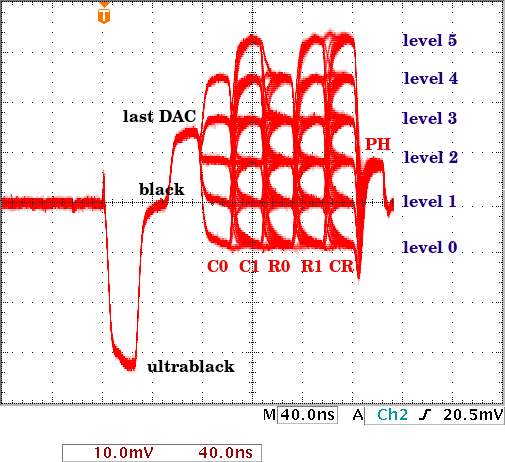
\includegraphics[width=\textwidth]{siganalog}
		\caption{Measured signal of several single pixel hits.}
		\label{panasig}
	\end{subfigure}
	\hfill
	\begin{subfigure}[b]{0.47\textwidth}
		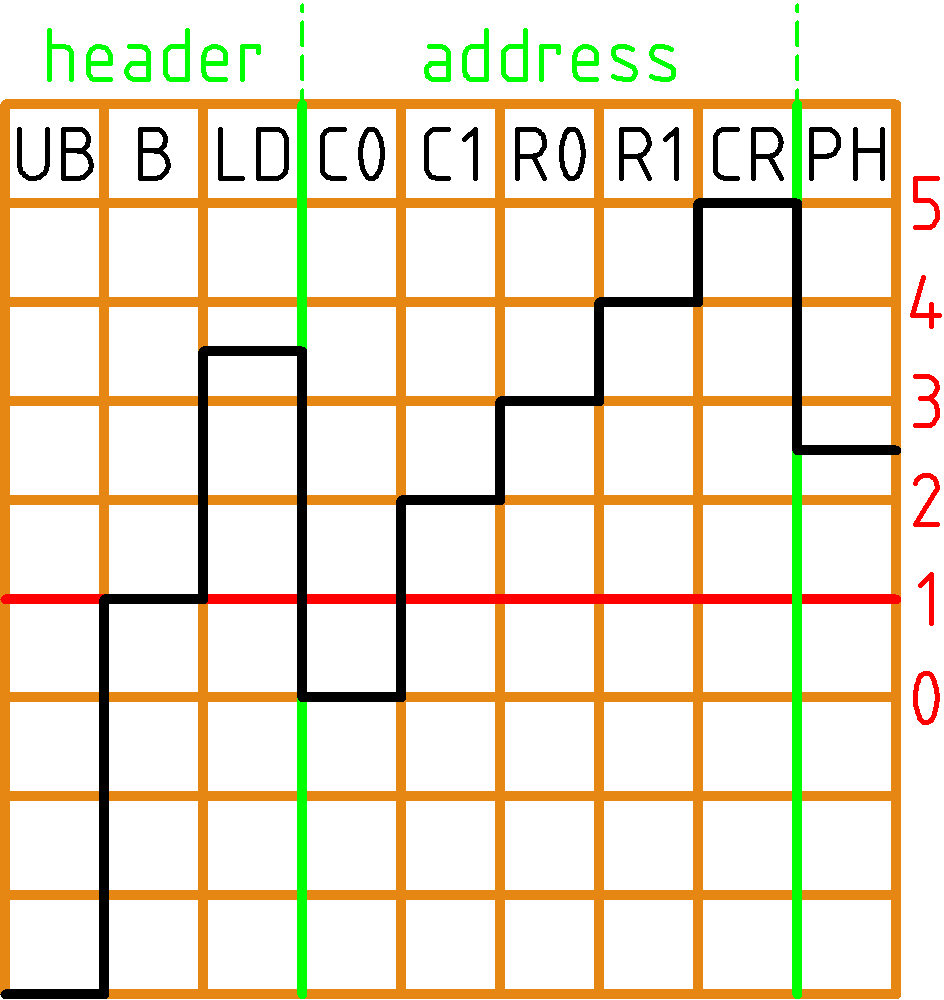
\includegraphics[width=\textwidth]{levels}
		\caption{Schematic signal of one single pixel hit.}
		\label{p7}
	\end{subfigure}
	\caption{Signals of the analogue \ac{ROC}}
	\label{procsig}
\end{figure}
Each single detector is set up to be read out in zero suppression mode, which means that for every single pixel hit, which exceed the threshold, following information is sent to the periphery: The time stamp of the current bunch crossing is written into the time stamp buffer and the analogue signals are written into the next free data buffer. This process happens autonomously and asynchronously for every double column. The information has to be kept until a trigger arrives. The pixel hits and the pulse height are read out at a frequency of $40\,$MHz, which corresponds to the \ac{LHC} bunch crossing frequency and are stored in the \ac{ROC} buffer for a certain amount of time: until the chip received a trigger or the buffer is full.\\
The \ac{ROC} may receive four different kinds of signals in order to readout the data:
\begin{enumerate}
	\item a trigger signal, length one clock cycle
	\item a calibrate signal, length two clock cycles
	\item a reset signal, length three clock cycles
	\item a token to collect the data
\end{enumerate}
The first three are sent over a single data line and are distinguished by the length of the signal. They are called \ac{CTR} in short.\\
Hits that were sent to the periphery are validated by the external trigger signal by comparing their corresponding time stamps with the delayed bunch crossing counter otherwise the hits are cleared. If the validation succeeds, the trigger counter is latched into the periphery, i.e. the double column is frozen and will not record further data until they are read out or the \ac{ROC} received the reset signal. Other double columns without validated hits remain active. When the latched trigger counter is matching the token counter the double column is set to readout mode and the trigger counter is incremented. As soon as the \ac{ROC} receives the token bit the the frozen double columns are read out and reset consecutively. Just before the token leaves the chip, the token counter is incremented as well. Illustrations of the trigger validation and the readout procedure are shown in \ar{pro}. \\
An example of an analogue readout with only the information of the the \ac{ROC} is shown in \ar{procsig}. To every readout the \ac{ROC} adds a header, which is three clock cycles long. It contains an \ac{UB} level that is a very low, negative level and serves as reference, a \ac{B} level that is the zero reference of the differential signal and a level that is called \ac{LD}, which either points to the value the last \ac{DAC} was set to or the value of the temperature sensor of the chip. For every single hit pixel the \ac{ROC} will provide five levels of position information and one level with information about the pulse height, which are added to the header. If no pixel was hit or the hits were not validated, the \ac{ROC} will send nothing but a header.\\
It is possible to read out several \ac{ROC}s with a single token. In that case the token is sent from on \ac{ROC} to the next collecting a header of each \ac{ROC} and the corresponding hit information s.t. a structure like Header/Hit/Header/Hit/Hit/Header/Header/Hit etc. will form. In my case the readout concerning sending and receiving \ac{CTR} and token is managed by an emulated \ac{TBM} from the \ac{DTB} connected to the \ac{ROC} that is described in \ar{sdtb}
\begin{figure}[ht]
	\centering
	\begin{subfigure}[b]{0.37\textwidth}
        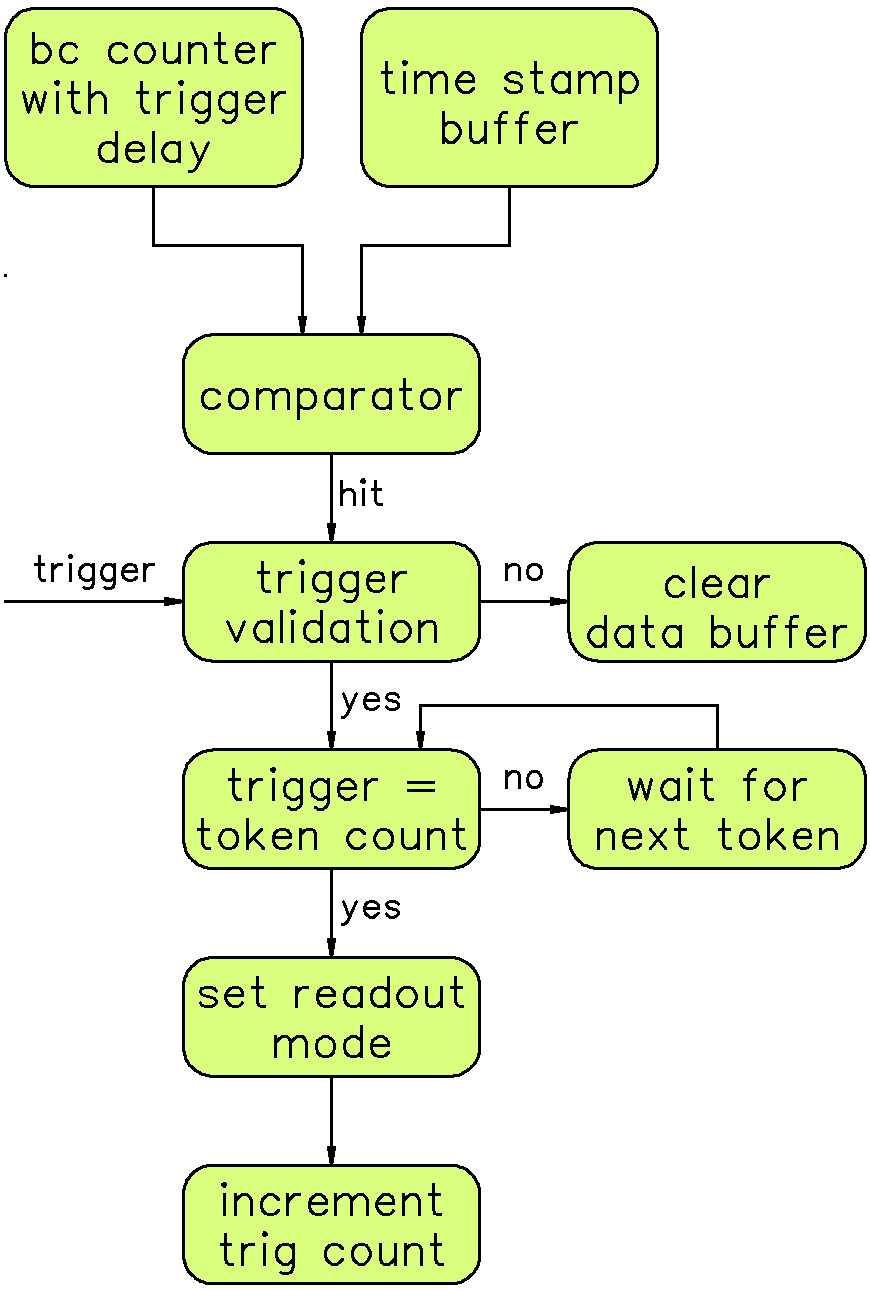
\includegraphics[width=\textwidth]{trigger}
		\caption{Trigger validation.}
		\label{ptrig}
	\end{subfigure}
	\hfill
	\begin{subfigure}[b]{0.57\textwidth}
		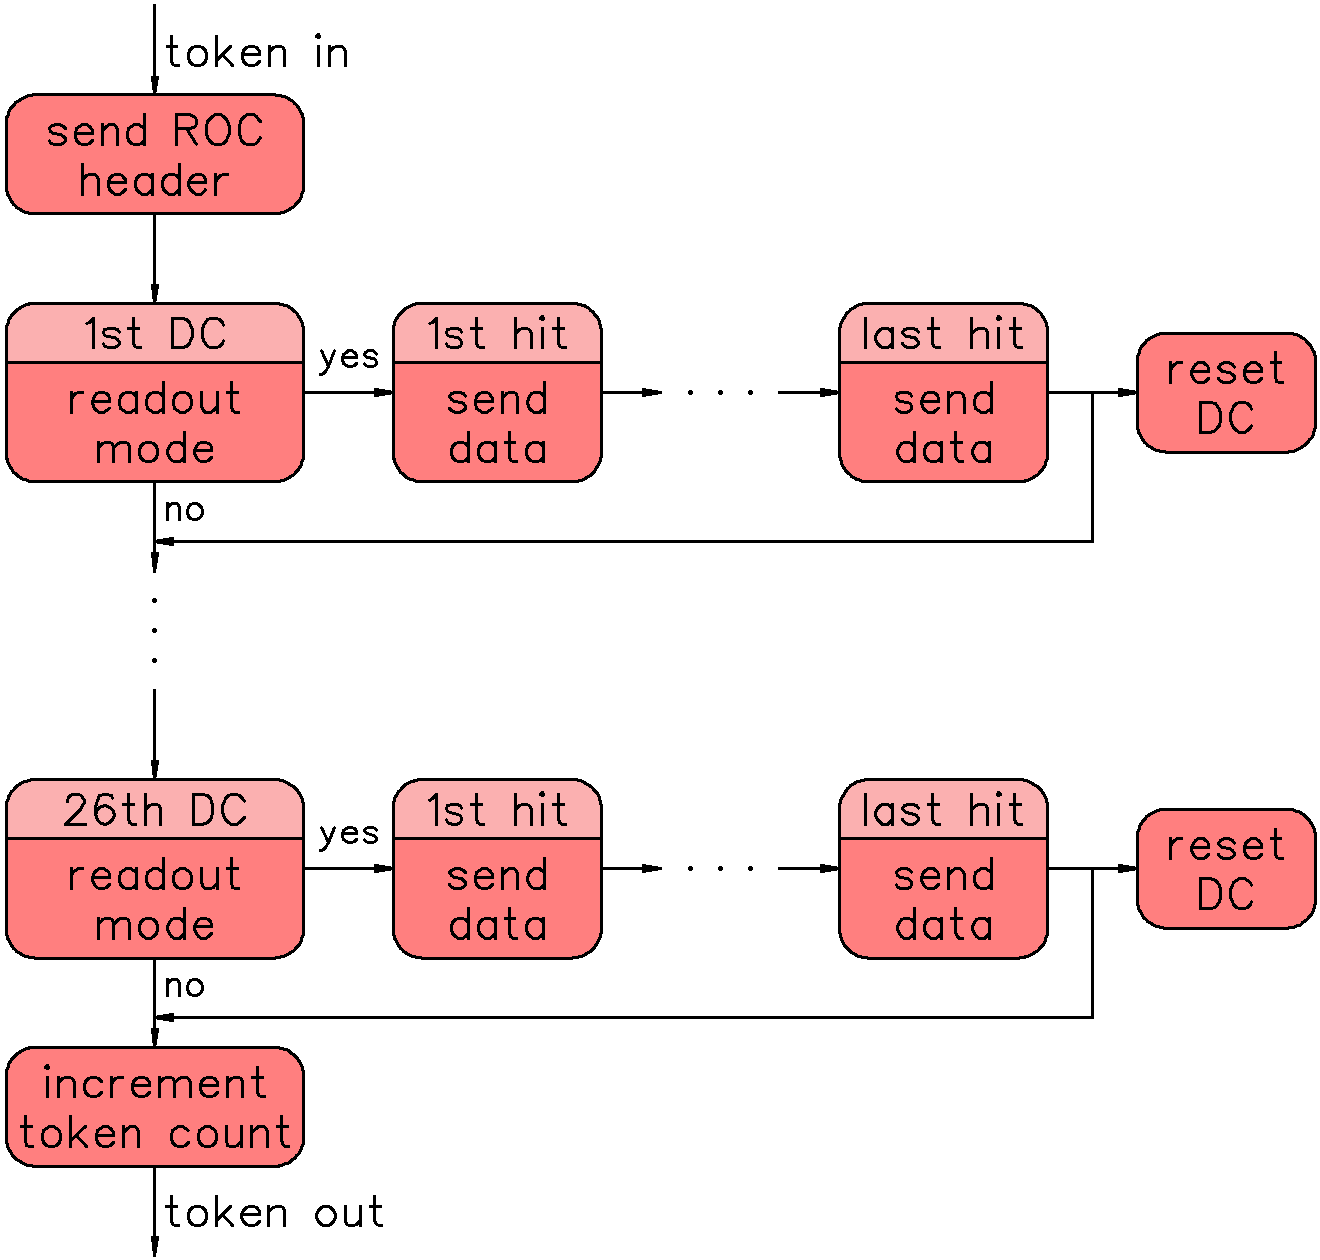
\includegraphics[width=\textwidth]{token}
		\caption{Readout procedure.}
		\label{ptok}
	\end{subfigure}
	\caption{Schematics of the readout of the \ac{ROC}. bc is short for bunch crossing and DC stands for double column}
	\label{pro}
\end{figure}
% ========================================================
\subsection{Digital Pixel Detector}\label{s23}
By motivation of the Phase I Upgrade of \ac{CMS} and an expected higher
\begin{wrapfigure}{r}{4.5cm}
	\vspace*{-10pt}
	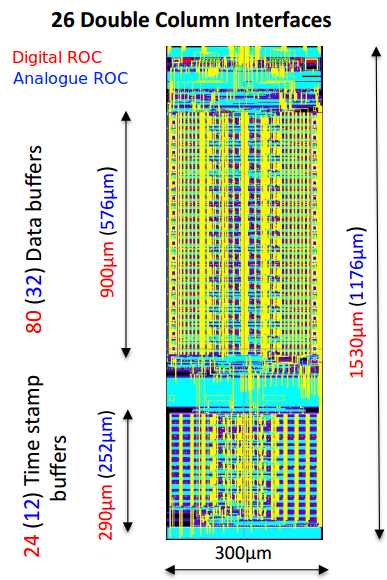
\includegraphics[width=4.4cm]{DigRocPeri}
	\caption{Double column interface of the digital \ac{ROC} \cite{hits}}
	\label{p12}
	\vspace*{-10pt}
\end{wrapfigure} 
luminosity a new \ac{ROC} was designed based on the analogue one. In principle both are still very similar. An overview of the differences can be found in \ar{t3}.\\
A limitation of the analogue \ac{ROC} was i.a. a limited buffer size for the Level 1 trigger latency. To overcome this problem the number of data buffers was increased from $32$ to $80$. To reduce the readout related dead times due to higher rate, the number of time stamp buffers doubled from $12$ to $24$. In addition the readout bandwidth had to be increased. This was done by switching to full digital readout by means of an on chip \ac{ADC}, new fast digital readout links, a \ac{PLL} to provide higher frequencies and some modifications to the control logic. The most important change regarding my thesis is the lower overall signal threshold that is required for a higher persistence of the chip \cite{hits}. This feature is indispensable for the low signals of diamonds. Going to lower thresholds was achieved by keeping the timewalk between the highest and lowest signal amplitudes within one clock cycle ($<16\,$ns) and due to reduced cross talk in the digital \ac{ROC} layout. Besides, the output of the fast-Or signal was removed from the digital \ac{ROC}.\\
For easier usage the number of \ac{DAC} parameters was reduced to $16$. There are now only one parameter (\textit{vwllpr} and \textit{vwllsh}) for the pre-amplifier and the shaper instead of two, there is no leakage current compensation any more and the six \ac{DAC} for the double column periphery, which are responsible for the shape of the pulse height vs. \textit{vcal} curve, were condensed into \textit{vibias\_bus} and \textit{phoffset}. A comparison of the \ac{DAC}s that changed can be found in \ar{tdacchange}.
\begin{table}[ht]
	\begin{tabularx}{\textwidth}{X|X|X}\noalign{\hrule height 2pt}
			 &\multicolumn{1}{c}{\textbf{psi46v2}}	&\multicolumn{1}{|c}{\textbf{psi46dig}}	\\\hline
		\ac{ROC} size					& $7.9\times9.8\,$mm	& $7.9\times10.2\,$mm 	\\
		Pixel size						& $100\times150\,\upmu$m& $100\times150\,\upmu$m\\
		Smallest radius					& $4.3\,$cm				& $2.9\,$cm				\\
		Settable \ac{DAC}s / registers	& $26$ / $3$			& $16$ / $2$			\\
		Power up condition				& not defined			& default values		\\
		Pixel charge readout			& analogue				& digitised, $8\,$bit	\\
		Readout speed					& $40\,$MHz				& $40\,$MHz				\\
		Time stamp buffer size			& $12$					& $24$					\\
		Data buffer size				& $32$					& $80$					\\
		Output buffer FIFO				& no					& yes					\\
		Double column speed				& $20\,$MHz				& $40\,$MHz				\\
		Metal layers					& $5$					& $6$					\\
		leakage current compensation	& yes					& no					\\
		In-time threshold				& $3500\,$e				& $<2000\,$e			\\
		\ac{PLL}						& no					& yes					\\
		Data loss at max 				& $\sim3.8\,$\% at  	& $\sim3\,$\% at		\\
		operating flux					& $120\,$Mhz/cm$^{2}$	& $580\,$Mhz/cm$^{2}$ \footnotemark[2]\\\noalign{\hrule height 2pt}
	\end{tabularx}					
	\caption{comparison between analogue and digital \ac{ROC} \cite{hits}}
	\label{t3}
\end{table}\no
\footnotetext[2]{valid for L1 version}
\begin{table}[ht]
	\begin{tabularx}{\textwidth}{c|l|l|X}
		\noalign{\hrule height 2pt}
		\textbf{\#} & \multicolumn{1}{l}{\textbf{analogue}} & \multicolumn{1}{|l}{\textbf{digital}}	& \multicolumn{1}{|l}{\textbf{comment}}\\\noalign{\hrule height 2pt}
		\multicolumn{4}{c}{\textbf{Analogue Signal (\ac{PUC})}}							\\\hline
		$05$ &	vleak				& $-$ 		& leakage current compensation removed			\\
		$06$ &	vrgpr				& $-$ 		& combined into vwllpr		\\	
		$07$ &	vwllpr				& vwllpr	&							\\
		$08$ &	vrgsh				& $-$		& combined into vwllsh		\\
		$09$ &	vwllsh				& vwllsh	&							\\\noalign{\hrule height 2pt}
		\multicolumn{4}{c}{\textbf{Double Column Periphery}}				\\\hline
		$13$ &	vibias\_bus 		& vibias\_bus	&						\\
		$14$ &	vbias\_sf			& $-$			&						\\
		$15$ &	voffsetop			& $-$			& the six periphery dacs\\
		$16$ &	vibiasop			& $-$			& were condensed into two \\
		$17$ &	voffsetroc			& phoffset		& 						\\
		$18$ &	vion				& $-$			&						\\\noalign{\hrule height 2pt}
		\multicolumn{4}{c}{\textbf{Control and Interface Block}}			\\\hline
		$19$ &	vibias\_dac 		& vcomp\_adc 	&						\\
		$20$ &	vibias\_ph 			& phscale 		& 						\\
		$21$ &	vibias\_roc 		& $-$			& removed				\\\noalign{\hrule height 2pt}
		\multicolumn{4}{c}{\textbf{Fast-OR Trigger (\ac{PUC})}}				\\\hline
		$22$ &	vicolor 			& vicolor	&							\\
		$23$ &	vnpix 				& $-$		& fast-OR removed			\\
		$24$ &	vsumcol	 			& $-$		& fast-OR removed			\\
		\noalign{\hrule height 2pt}
	\end{tabularx}					
	\caption{Different \ac{DAC}s for analogue and digital \ac{ROC}}
	\label{tdacchange}
\end{table}\no
% ========================================================
\subsection{\ac{DTB}}\label{sdtb}
The psi46 \ac{DTB} is the interconnect between a computer and the \ac{ROC}. Usually the analogue chips were operated with an \ac{ATB}, which has some major disadvantages in comparison with the \ac{DTB}. E.g. it has only a limited amount of data it can save, s.t. during beam tests one could only take runs of approximately five minutes until the buffer was full. The more flexible, user-friendly and more extensive readout software is another advantage in my opinion. One of the achievements of this thesis is the possibility to operate analogue chips as well as digital chips with the \ac{DTB}.\\
The \ac{DTB} connects via an adapter to the \ac{ROC}. It has two interfaces to a computer of which the ethernet is not implemented yet, s.t. the only option is the USB. Once connected to the chip and a computer, the \ac{DTB} is completely controlled with the software called pXar including the internal \ac{FPGA} which has its own firmware written by Beat Meier at \ac{PSI}. By now there more than twenty iterations of this firmware, which can be easily upgraded via USB. During my thesis I was using the the versions from $4.0$ to $4.2$.\\
It is possible to read out several signals of the \ac{DTB}. For that purpose there are two digital and two differential analogue LEMO outputs.\\
Furthermore the \ac{DTB} has an inputs for an external clock and trigger, which only accepts \ac{TTL} signals. The height of the external trigger signal has to be at least $3\,$V to guarantee stability. Since these inputs are not terminated by $50\,\Upomega$ it is important to terminate incoming signals at the input to avoid reflections inside the cables. The \ac{DTB} has also an \ac{HV} input that is able to distribute the \ac{HV} to the \ac{ROC} via an adapter in order to bias the the sensor.\\
The \ac{DTB} or rather its \ac{FPGA} is emulating the \ac{TBM} which is, as the name suggests in charge of token as well of the external trigger sent to the \ac{ROC}. Once it received and processed an external trigger it will send a trigger and a token in short succession to the \ac{ROC}. To keep track of the sent signals it has $4\,$ trigger and token counter as well, the trigger counter is incremented once a trigger is sent the token counter once a token is received. When the \ac{TBM} gets the token with the data stream back it adds information in form of a header and trailer to the data package. The header contains an $8-$bit event number and information about the trigger position inside the clock cycle, the trailer contains i.a. stack counter that gives information about the number of events that are stacked inside the \ac{TBM}. A stack arises if the \ac{TBM} sends out more triggers than it receives tokens, whereas the maximum stack is $16$, which is equivalent the maximum of the trigger and token counter.\\
\begin{figure}[ht]
	\centering
	\begin{subfigure}[b]{0.47\textwidth}
        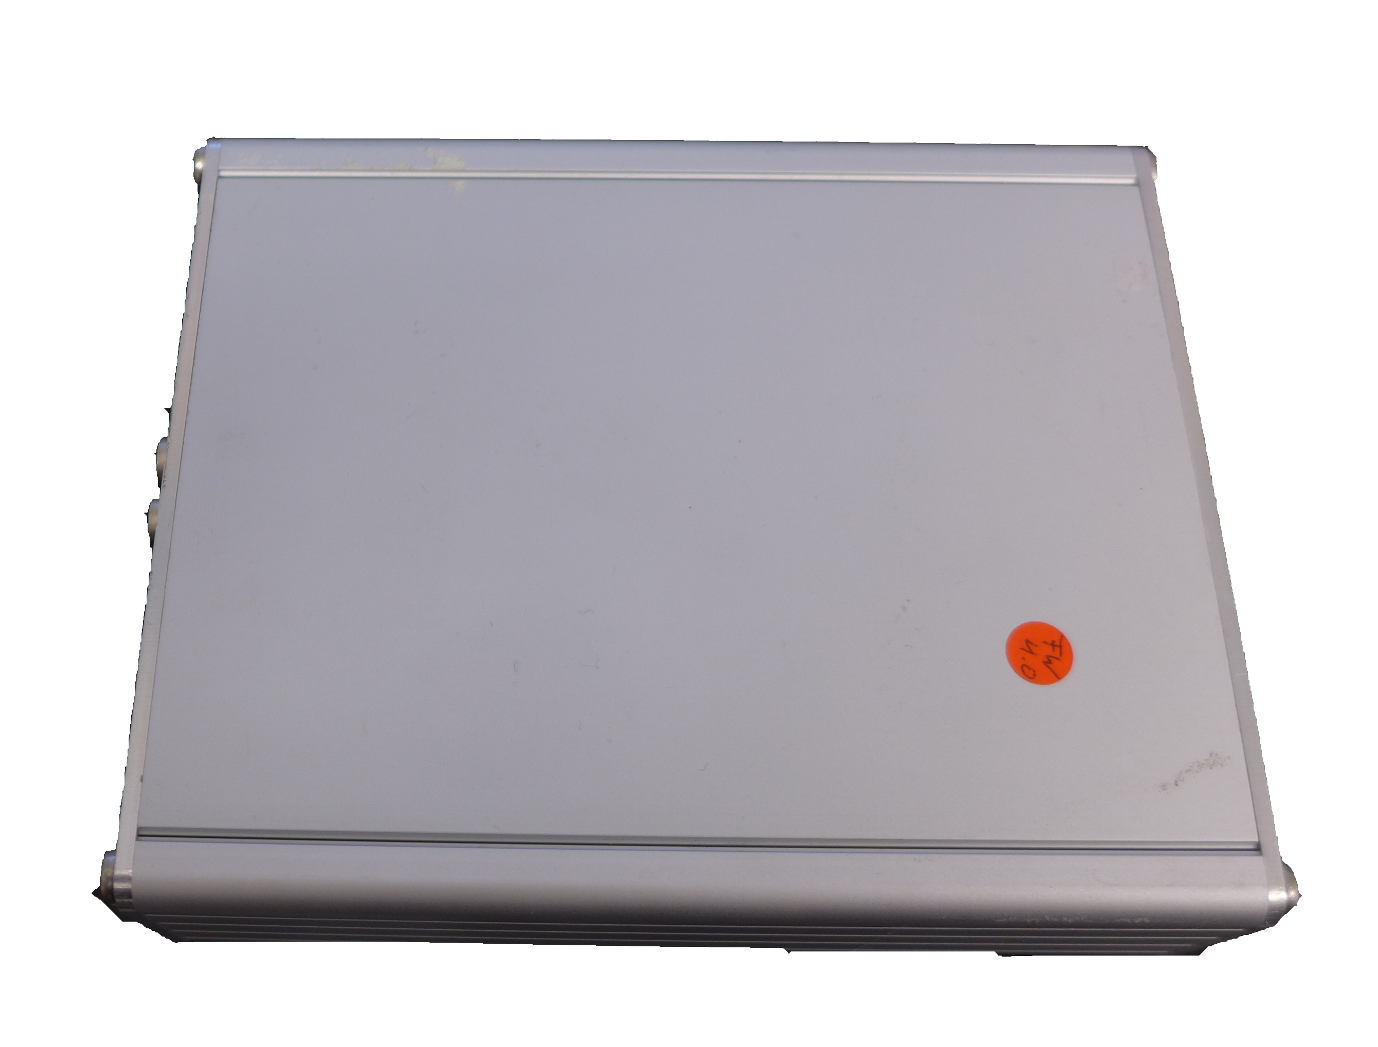
\includegraphics[width=\textwidth]{DTB}
		\caption{Top view.}
		\label{p10}
	\end{subfigure}
	\hfill
	\begin{subfigure}[b]{0.47\textwidth}
		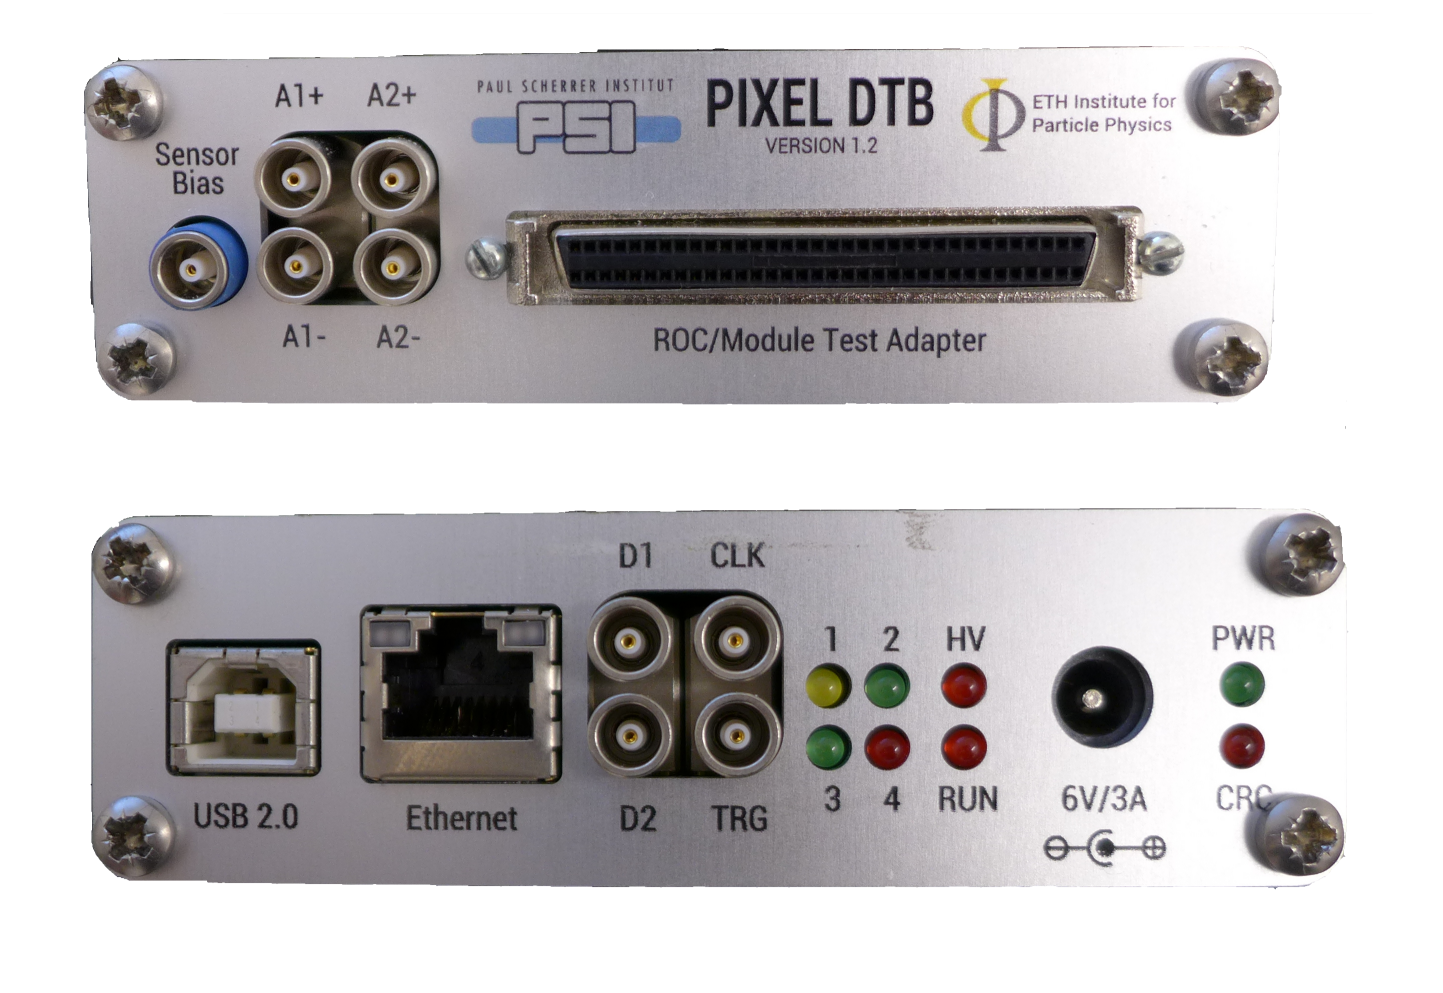
\includegraphics[width=\textwidth]{DTB-Sides}
		\caption{Front and backside.}
		\label{p11}
	\end{subfigure}
	\caption{Photographs of the \ac{DTB}.}
	\label{pdtb}
\end{figure}